\mysubsubsection{Stereo}

\noindent We have chosen 7 images with the resolution of $695\times555$
from the Book sequence of Middlebury stereo dataset~\cite{middlebury_stereo} for our
experiment. The number of disparity labels is
set to 256.
%
Since the order of labels is important for the expansion techniques,
we have used the same random order for all algorithms to avoid any
bias.
%
% In PAE, SF-MF, SF-SS and SF algorithms, the proposal generator in each
% thread can only generate constant-label proposals within a evenly split
% subset of all labels.

Fig.~\ref{fig:stereo_global} compares the converegence rate of the
competing methods. Note that we define the energy of a multi-threading
system to be the energy of the best solution found so far.
%

\begin{figure}[tb]
\centering
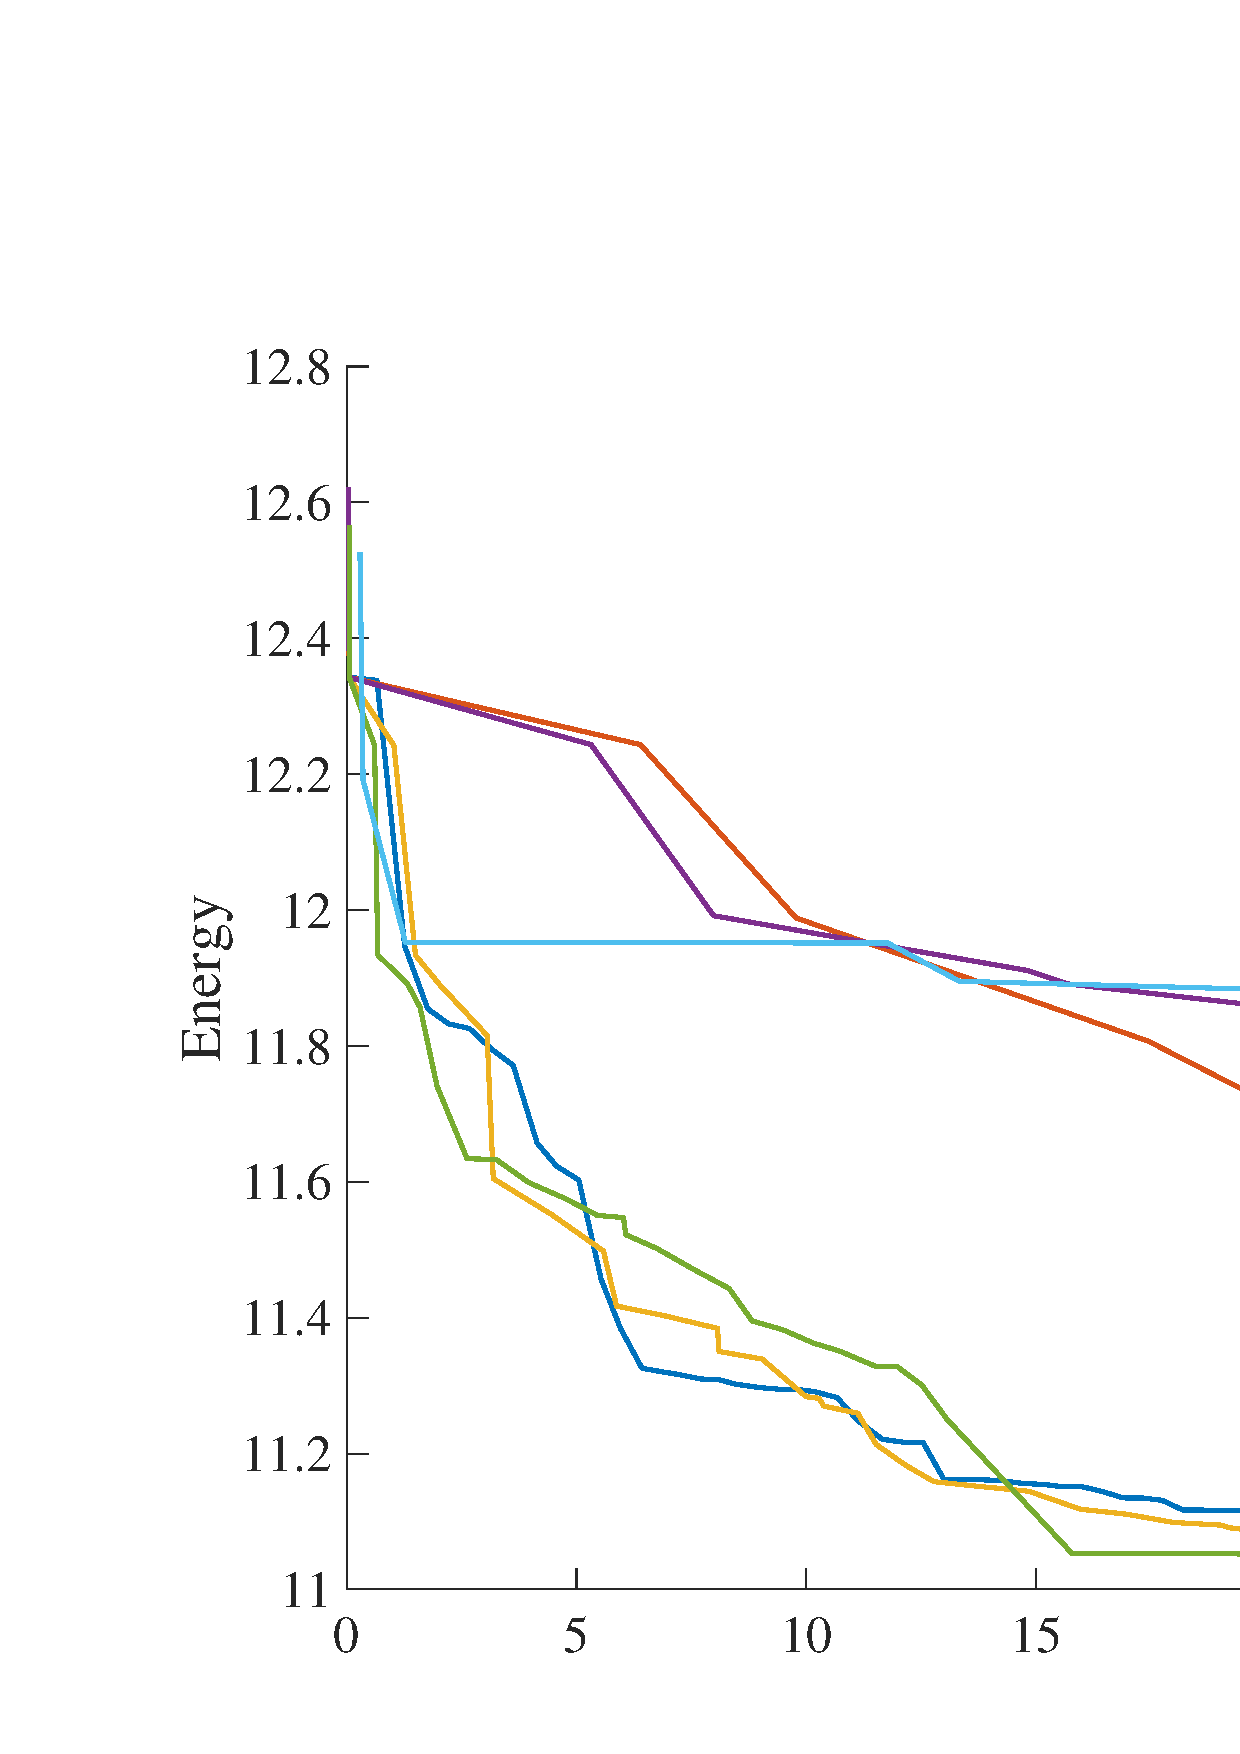
\includegraphics[width=0.8\textwidth]{figure/stereo_global.png}
\caption{Energy plots for the stereo problem. The energy is in the log
scale. For a multi-threading algorithm, the energy at a given moment is
defined to be the best solution so far.}
\label{fig:stereo_global}
\end{figure}
%

One unusual outcome is that Sequential Alpha Expansion and Parallel
Alpha Expansion (PAE) have the same convergence speed, indicating that
the stereo problem is a very easy one.
%This is well known in a community and this fact was rather expected.
Our approaches with multi-way fusion (SF-SS or SF) are the slowest kind,
because the TRW-S for multi-way fusion is slower than multiple Alpha
Expansion steps, and this stereo problem is too easy to gain benefits
through mulit-way fusion.
%
%Another interesting observation is that the Hierarchical Fusion can
%achieve good energy only when they merge solutions at the top of the
%tree.
%
%  both PAE and SF-MF converge faster
% than sequential method. However, since fusing solutions with multiple
% labels by QPBO is slower than a single $\alpha$-expansion, PAE method
%
% Finally, the line of hierarchy fusion only makes
% jump when fusing on root node of the tree. This is because any fusion
% step on non-root nodes only have partial label information.
%We recoreded both single thread energy and system energy against
%time.
%
Fig. \ref{fig:stereo_threads} shows the energy plot per thread for
SF-MF (ours) and PAE. With solution sharing, the energy of a single
thread in SF-MF decreases more uniformly, while in PAE the energy
makes dramatic decrease at the final fusion.
%
%The graph for PAE again confirms that the
%stereo is an easy problem, because all the threads are quickly
%converging to a solution before the final sequential fusion.
%shows the per-thread energy
%minimization process in SF-MF and PAE. The per-thread energy in SF-MF
%architecture decreases more uniformly than that of PAE. In the
%scenario where we need to query the best solution so far before the
%whole optimization converges, SF-MF architecture is a better choice.

\begin{figure}[tb]
\includegraphics[width=\columnwidth]{figure/stereo_threads.png}
\caption{Energy plots per thread for the stereo proble for SF-MF (left) and
Parallel Alpha Expansion (right).
} \label{fig:stereo_threads}
\end{figure}

For an easy optimization problem such as stereo with strong unary terms
and submodular pairwise terms, our full architecture with solution
sharing and multi-way fusion actually makes convergence slower due to the
overhead of fusion and multi-threading.




% over-sophisticated fusion algorihtm and multi-threading
% overhead. However, we can easily configure the architecture to make it
% better fit the problem, e.g. turn off multiway fusion and/or solution
% sharing.





% We define the energy of
% a parallel optimization system at a certain time as the minimum energy
% of all threads at that time.
